\documentclass[a4paper,12pt]{article} % тип документа

% Поля страниц
\usepackage[left=2.5cm,right=2.5cm,
    top=2cm,bottom=2cm,bindingoffset=0cm]{geometry}
    
%Пакет дял таблиц   
\usepackage{multirow} 
    
%Отступ после заголовка    
\usepackage{indentfirst}


% Рисунки
\usepackage{floatrow,graphicx,calc}
\usepackage{wrapfig}



% Создаёем новый разделитель
\DeclareFloatSeparators{mysep}{\hspace{1cm}}

% Ссылки?
\usepackage{hyperref}
\usepackage[rgb]{xcolor}
\hypersetup{				% Гиперссылки
    colorlinks=true,       	% false: ссылки в рамках
	urlcolor=blue          % на URL
}


%  Русский язык
\usepackage[T2A]{fontenc}			% кодировка
\usepackage[utf8]{inputenc}			% кодировка исходного текста
\usepackage[english,russian]{babel}	% локализация и переносы




% Математика
\usepackage{amsmath,amsfonts,amssymb,amsthm,mathtools}

%%% Дополнительная работа с математикой
\usepackage{amsmath,amsfonts,amssymb,amsthm,mathtools} % AMS
\usepackage{icomma} % "Умная" запятая: $0,2$ --- число, $0, 2$ --- перечисление


% Что-то 
\usepackage{wasysym}


\begin{document}
\floatsetup[table]{capposition=top}
\begin{center}
	\footnotesize{ФЕДЕРАЛЬНОЕ ГОСУДАРСТВЕННОЕ АВТОНОМНОЕ ОБРАЗОВАТЕЛЬНОЕ 			УЧРЕЖДЕНИЕ ВЫСШЕГО ОБРАЗОВАНИЯ}\\
	\footnotesize{МОСКОВСКИЙ ФИЗИКО-ТЕХНИЧЕСКИЙ ИНСТИТУТ\\(НАЦИОНАЛЬНЫЙ 			ИССЛЕДОВАТЕЛЬСКИЙ УНИВЕРСИТЕТ)}\\
	\footnotesize{ФАКУЛЬТЕТ ОБЩЕЙ И ПРИКЛАДНОЙ ФИЗИКИ\\}
	\hfill \break
	\hfill \break
	\hfill \break
	\hfill \break
\end{center}


\begin{figure*}[h]
    \centering
    \includegraphics*[width=10cm,height=7cm,keepaspectratio]{mipt_eng_text_png.png}
    \label{fig:my_label}
\end{figure*}


\begin{center}   
    \hfill \break
	\hfill \break
	\hfill \break
	\large{Лабораторная работа № 5.11.8\\ \hfill \break\Large{Экспериментальная проверка закона Видемана-Франца}}\\
	\hfill \break
	\hfill \break
	\hfill \break
	\hfill \break
	\begin{flushright}
		Баранов Даниил\\
		Группа Б02-103
	\end{flushright}
	\hfill \break
	\hfill \break
	\hfill \break
\end{center}
\hfill \break
\hfill \break
\hfill \break
\begin{center}
	Долгопрудный, 2024 г.
\end{center}
\thispagestyle{empty}

\newpage

\textbf{Цель работы:} экспериментально определить величины постоянной Лоренца $\displaystyle L=\frac{\kappa}{T\sigma}$ (здесь $\kappa$ – коэффициент теплопроводности, $\sigma$ – проводимость, а $T$ —
абсолютная температура) при комнатной температуре для нескольких распространенных металлов и сплавов: меди, латуни, алюминия, дюралюминия.

\textbf{В работе используется:} два вольтметра В7-78/1; два источника постоянного тока INSTEK GPR30H10D; 
вольтметр В7-38; экспериментальная ячейка с исследуемым образцом.

\section{Теоретическая справка}

В постоянную Лоренца входят удельные характеристики материала: проводимость и теплопроводность. Их вычисление требует точного учёта геометрии образца, что является источником дополнительной погрешности. Необходимо отметить, что прецизионное измерение проводимости (сопротивления) и теплопроводности, вообще говоря, требуют разной геометрии эксперимента. Для измерения сопротивления предпочтительно иметь длинный однородный проводник с заметным сопротивлением. При измерении теплопроводности важно избежать неконтролируемых потерь тепла, для чего предпочтителен образец с минимальной площадью боковых стенок. В то же время, во многих случаях в реальном эксперименте желательно проводить измерения разных величин на одном и том же образце.

Используемая в этой работе схема измерения моделирует этот подход (измерение разных физических величин, входящих в конечный ответ, на одном образце), а также позволяет исключить влияние геометрии образца за счёт выбора геометрии эксперимента.

Исследуемыми образцами являются металлические стержни диаметром $3.5-5$ мм и длиной около $50$ мм, изготовленные из различных распространённых металлов и сплавов: меди, латуни (сплава меди и цинка с незначительным добавлением других добавок, типичное содержание меди $60-80\%$), алюминия и дюралюминия (сплав, содержащий $94\% $ Al, $4\%$ Cu, $1\%$ Mg и другие добавки). На образце выбираются две измерительные точки, между которыми измеряются и электрические, и тепловые свойства: и падение напряжения при измерении сопротивления, и разность температур при измерении теплопроводности. Таким образом, сопротивление и теплопроводность измеряются на одном и том же фрагменте стержня (с точностью до погрешности монтажа потенциометрического контакта и спая термопары).

Полное сопротивление цилиндрического фрагмента между измерительными точками $\displaystyle  R=\frac{l}{\sigma S}$ , где $l$ — длина фрагмента, а $S$ — площадь сечения. Сопротивлениеизмеряется по стандартной четырёхконтактной схеме: через образец пропускается известный ток через токоподводящие контакты на концах образца и измеряется падение напряжения между измерительными точками. Так как в цепи идеального вольтметра ток не течёт, такая схема позволяет полностью исключить сопротивления контактов, важные, например, для покрытых оксидной плёнкой алюминиевых образцов.

Перепад температур $\Delta T$ между измерительными точками в отсутствие потерь на боковых стенках при выделении мощности $P$ на одном из концов стержня задаётся уравнением
$\displaystyle  \frac{P}{S}= \kappa \frac{\Delta T}{l}$. Для исключения потерь тепла при измерении теплопроводности образец
окружается коаксиальным экраном, на котором поддерживается тот же градиент температур, что и на образце. При этом, пренебрегая конвекцией, радиального потока тепла от образца к экрану нет.

Тогда для числа Лоренца получаем:
$\displaystyle L=\frac{\kappa}{T\sigma}=\frac{PR}{\Delta T} \times \frac{1}{T}$, то есть геометрия образца в ответ явно не входит, а входят только
реально измеряемые величины: сопротивление, выделяемая на нагревателе мощность, перепад температур.

\section{Экспериментальная установка}

\subsection{Экспериментальная ячейка}

Эскиз экспериментальной ячейки и схема электрических цепей ячейки показаны на рисунке \ref{ust1}. Фотография одной из ячеек показана на рисунке \ref{ust2}.

В различных экспериментальных ячейках установлены образцы из разных металлов. Ячейки маркированы цифрами на наклейке на основании и выбитыми цифрами на верхней крышке экрана и боковой стороне основания. В нашей работе в качестве исследуемого образца выступал латунный стержень.

Основание ячейки установлено на радиаторе, так что его температура поддерживается примерно равной комнатной. В основание крепится образец: стержень из одного из металлов, существенные геометрические параметры образца: диаметр образца $d$ -- 5 мм, расстояние между измерительными точками $l$ -- 50 мм. На второй конец образца установлен нагреватель, изготовленный из намотанного на медный каркас высокоомного провода. В образце перпендикулярно к его оси сделано два отверстия малого диаметра, в которых монтируются измерительные контакты: потенциометрические контакты для измерения сопротивления и спаи термопары для измерения перепада температур. В медный и латунный образцы потенциометрические контакты впаяны, в алюминиевом и дюралюминиевом образцах в отверстия ввёрнуты латунные винты, к которым припаяны потенциометрические контакты.

Образец окружён коаксиальным экраном, нижний конец которого термализуется с тем же основанием, что и образец, а на верхнем конце установлен нагреватель (также изготовленный из высокоомного провода) на одном уровне с нагревателем образца. Перепад температур между «горячими» концами образца и экрана контролируется отдельной термопарой. В ходе эксперимента подбирается мощность нагрева экрана так, чтобы перепад температур (термоЭДС этой термопары) обращался в ноль.

При измерении сопротивления образца измерительный ток пропускается через весь образец, токоведущие провода крепятся к основанию ячейки и к корпусу нагревателя образца.

Для уменьшения количества проводов и количества используемых приборов некоторые цепи экспериментальной ячейки коммутируются при переключении между режимами измерения сопротивления и теплопроводности. Переключатели установлены на основании ячейки, оба переключателя во время эксперимента должны находиться в одинаковом положении («измерение сопротивления» или «измерение теплопроводности»).

\begin{figure}[H]
    \centering
    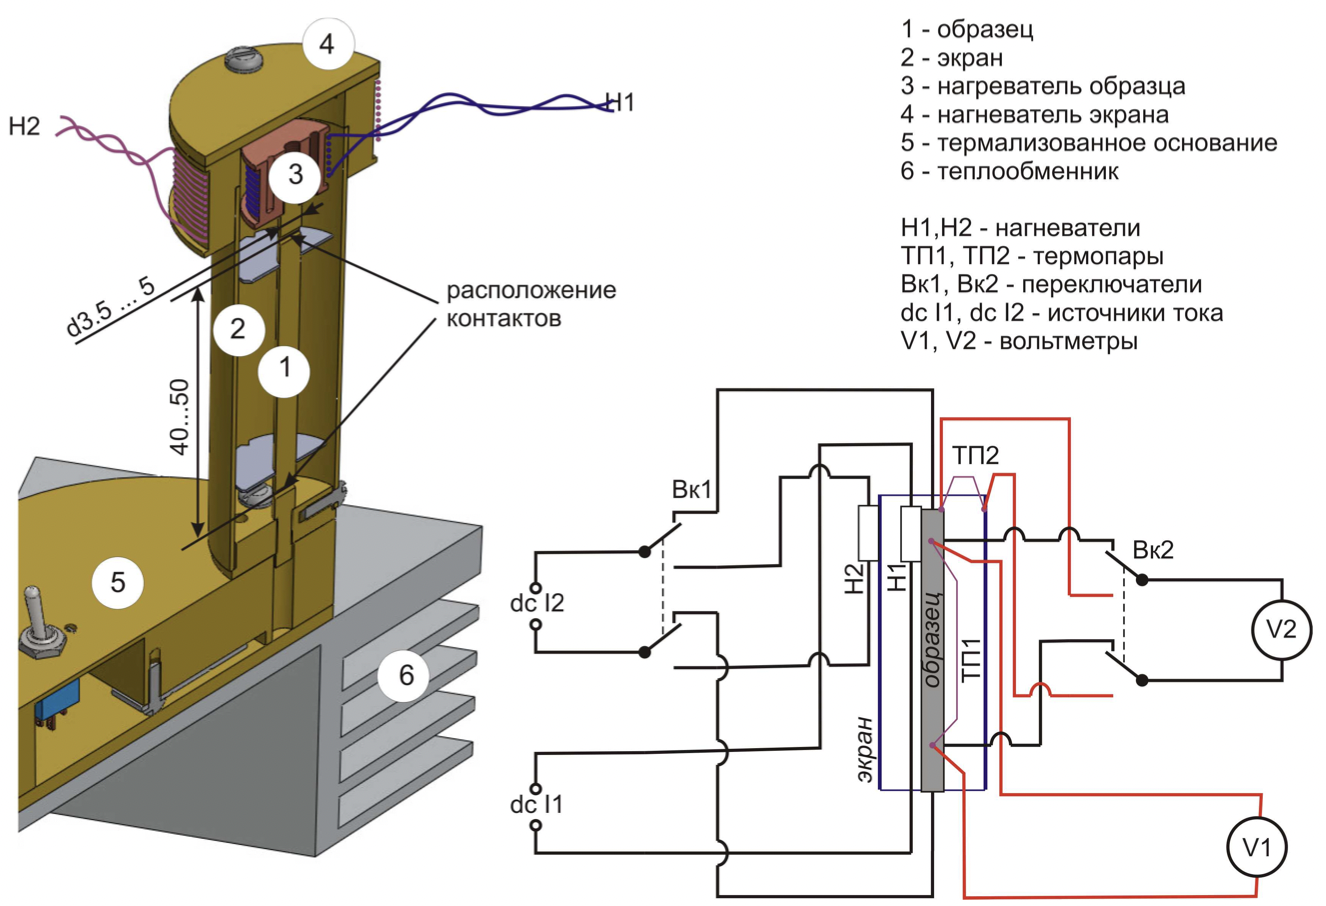
\includegraphics[width = 1\textwidth]{5.11.8/ust1.png}
    \caption{Эскиз экспериментальной ячейки и схема электрических цепей экспериментальной ячейки. На схеме переключатели Вк1 и Вк2 показаны в положении измерения сопротивления}
    \label{ust1}
\end{figure}

\begin{figure}[H]
    \centering
    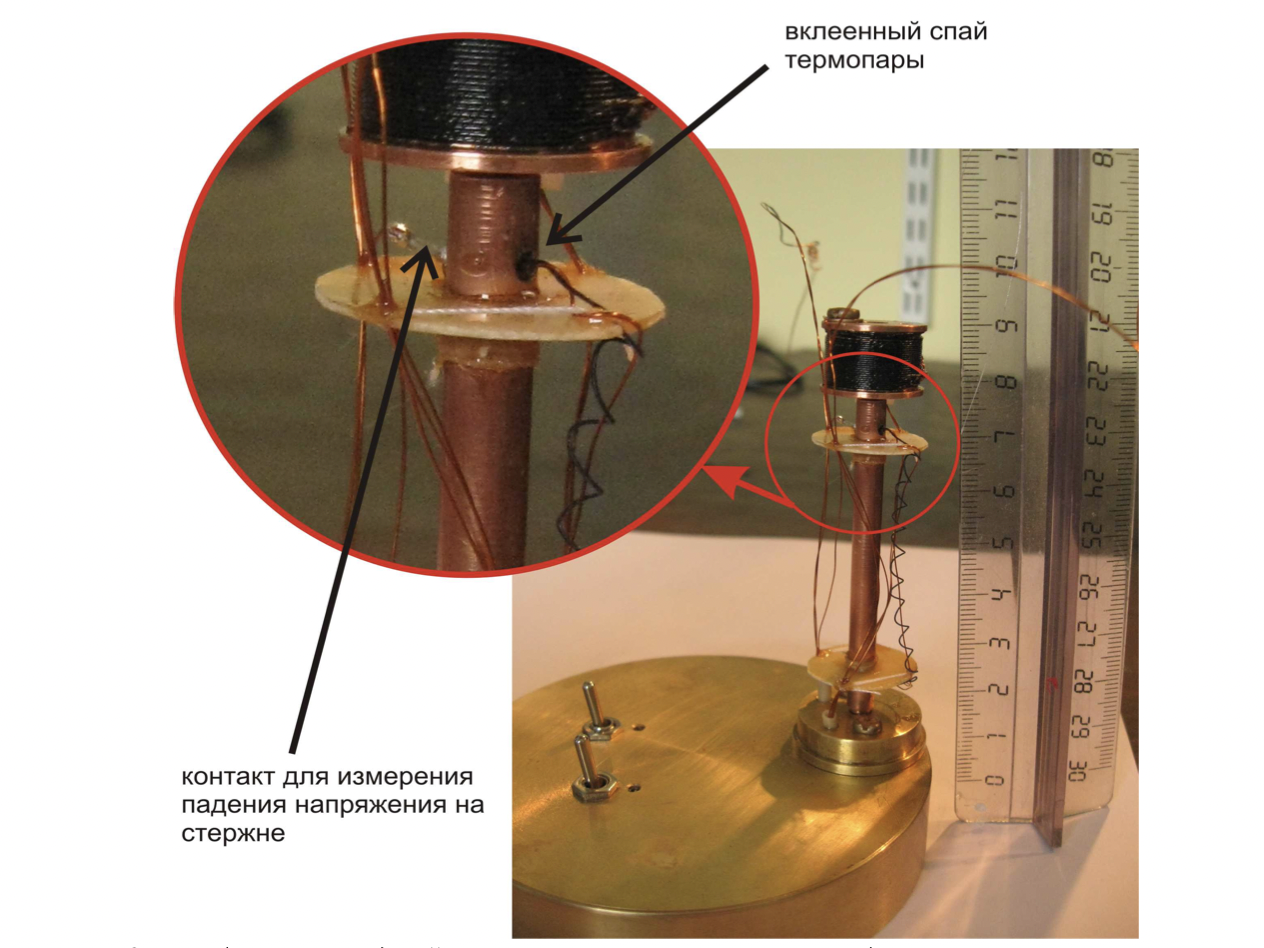
\includegraphics[width = 1\textwidth]{5.11.8/ust2.png}
    \caption{Изображение одной из экспериментальных ячеек без компенсирующего экрана. На увеличенном фрагменте показан один из измерительных контактов}
    \label{ust2}
\end{figure}

\subsection{Измерительная установка}

Фотография установки с подключенной экспериментальной ячейкой показана на рисунке \ref{ust3}.

В эксперименте используется два вольтметра В7-78/1, используемых для измерения термоЭДС термопар при измерении теплопроводности и падения напряжения при измерении сопротивления, два источника постоянного тока INSTEK GPR30H10D, используемые для питания нагревателей экрана и образца при измерении теплопроводности и для пропускания тока через образец при измерении сопротивления, и вольтметр В7-38, используемый для точного измерения напряжения на нагревателе образца при измерении теплопроводности.

В зависимости от положения переключателей на основании ячейки один из источников используется для пропускания тока через образец или для нагрева экрана, а один из вольтметров — для измерения падения напряжения на образце или для измерения термоЭДС между образцом и экраном. На вольтметрах и источниках наклеены этикетки на лицевой панели, указывающие к чему они подключены.

Вольтметр используется для измерения падения напряжения на образце при измерении сопротивления и термоЭДС на термопарах.

Штекеры проводов от ячейки втыкаются для измерения напряжения в правые гнёзда на лицевой панели. В некоторых случаях может быть удобно поменять штекеры местами для изменения полярности индицируемого напряжения.

Вольтметр должен находиться в режиме измерения постоянного напряжения, шкала 100 мВ. Этот режим индицируется строкой «Range:100 mVDC» на экране вольтметра.

Количество индицируемых разрядов на экране вольтметра регулируется кнопками «Установка» (треугольные кнопки на правой стороне лицевой панели). Необходимо установить максимальное число знаков (четыре знака после запятой, младший разряд 0.1 мкВ).

Переключатель входных каналов «Фронт/Тыльн» (круглая кнопка рядом с гнёздами подключения проводов) должен находиться в отжатом положении («Фронт»).

\begin{figure}[H]
    \centering
    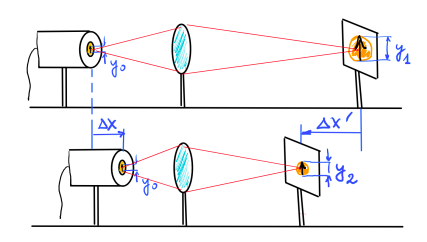
\includegraphics[width = 0.5\textwidth]{5.11.8/ust3.png}
    \caption{Экспериментальная установка}
    \label{ust3}
\end{figure}

\subsection{Термопары}

В работе используются медь-константановые термопары. При комнатной температуре чувствительность термопары равна 43 мкВ/К.

\section{Измерения и обработка данных}

Для начала была снята ВАХ образца для определения сопротивления. Полученные данные приведены в таблице \ref{vah1}.

\begin{table}[H]
    \centering
    \begin{tabular}{|c|c|c|c|}
    \hline
        \multicolumn{2}{|c|}{Начальная полярность} & \multicolumn{2}{|c|}{Другая полярность} \\ \hline
        $I$, mA & $V$, mkV & $I$, mA & $V$, mkV \\ \hline
        76  & 15  & 61 & 7  \\ \hline
        193 & 34 & 116 & 16 \\ \hline
        230 & 40 & 198 & 29 \\ \hline
        282 & 47 & 252 & 38 \\ \hline
        342 & 56 & 298 & 45 \\ \hline
        405 & 66 & 341 & 51 \\ \hline
        476 & 77 & 384 & 59 \\ \hline
        526 & 85 & 432 & 66 \\ \hline
        580 & 94 & 491 & 75 \\ \hline
    \end{tabular}
    \caption{Данные, полученные в процессе снятия ВАХ}
    \label{vah1}
\end{table}

По полученным данным можно построить график (рис. \ref{graph}) и найти сопротивление по углу наклона. Оно составило $R = 157,8 \pm 0,2$ мкОм.

\begin{figure}[H]
    \centering
    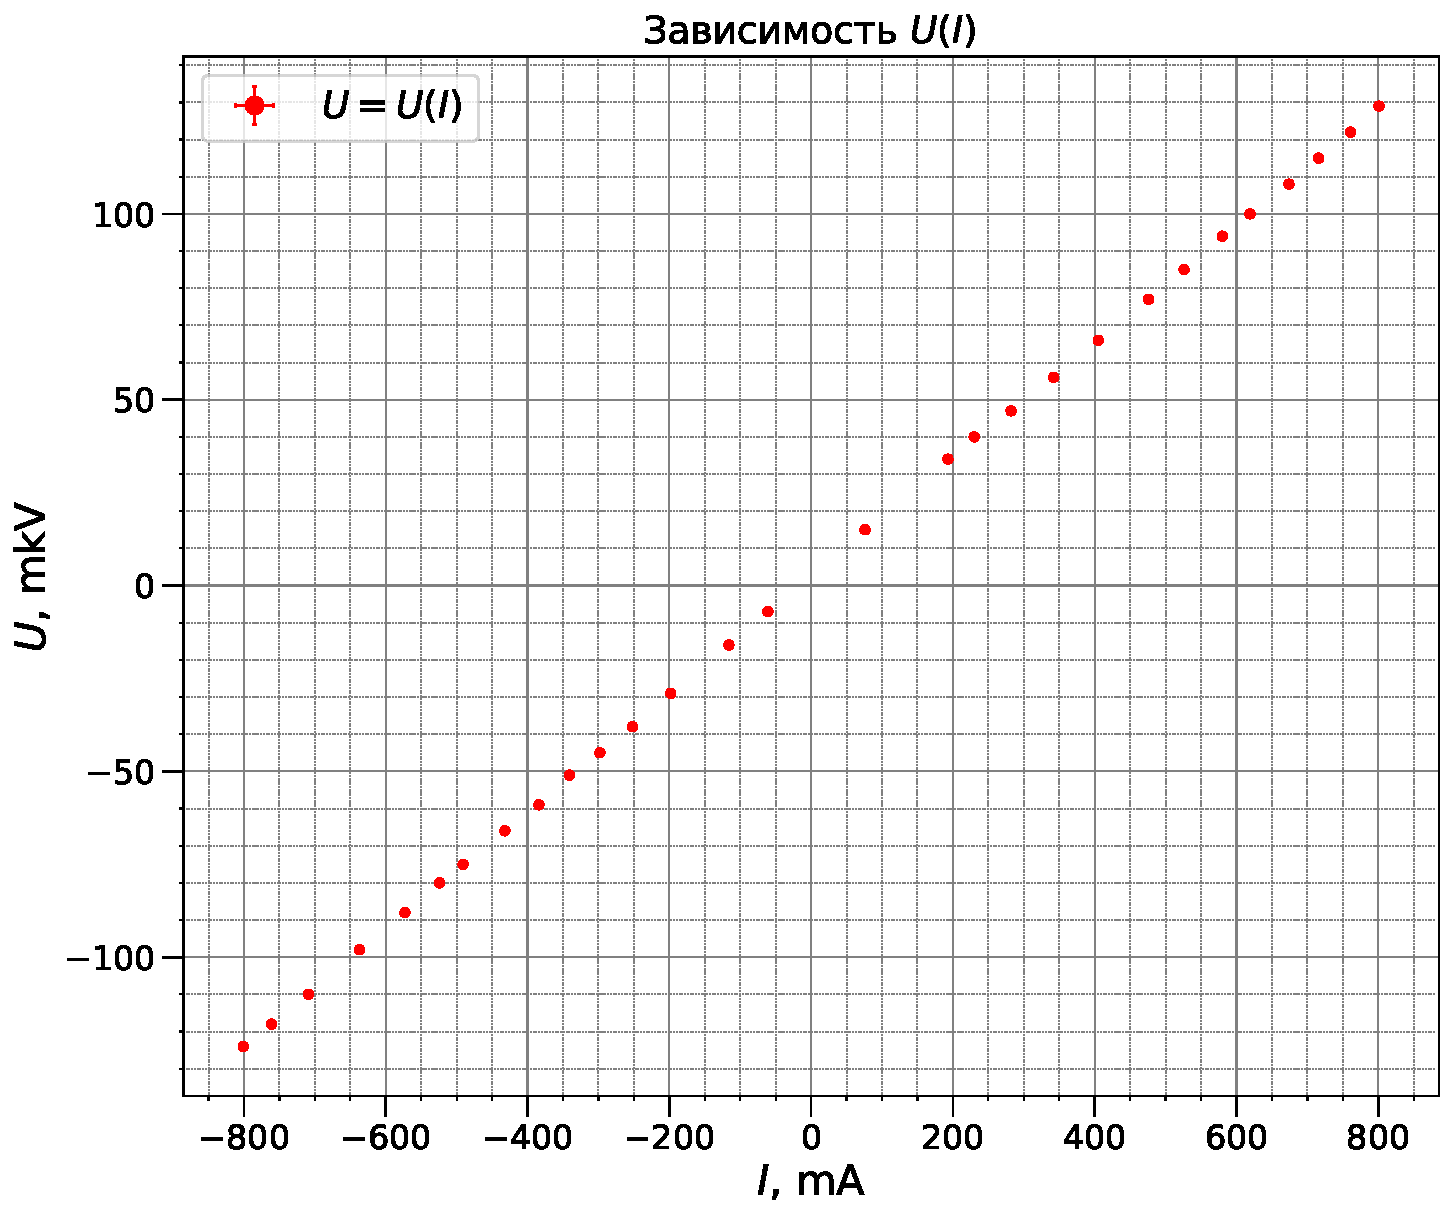
\includegraphics[width=1\textwidth]{5.11.8/U(I).pdf}
    \caption{ВАХ стержня}
    \label{graph}
\end{figure}

Далее, для измерения коэффициента теплового сопротивления была измерена зависимость $\Delta T(P)$. Полученные данные, необходимые для вычислений, приведены в таблице \ref{table}.

\begin{table}[H]
    \centering
    \begin{tabular}{|c|c|}
    \hline
        $P$, нВт & $\Delta T$, К \\ \hline
        150 & 4,19 \\ \hline
        352 & 5,88 \\ \hline
        400 & 6,30 \\ \hline
        450 & 9,09 \\ \hline
        500 & 11,42 \\ \hline
        897 & 14,42 \\ \hline
    \end{tabular}
    \caption{Данные для нахождения теплового сопротивления}
    \label{table}
\end{table}

По полученным данным был построен график (рис. \ref{graph1}) и вычислен коэффициент теплового сопротивления, который составил $A = 14.6 \pm 2.7 \cdot 10^{6}$ ед. СИ.

\begin{figure}[H]
    \centering
    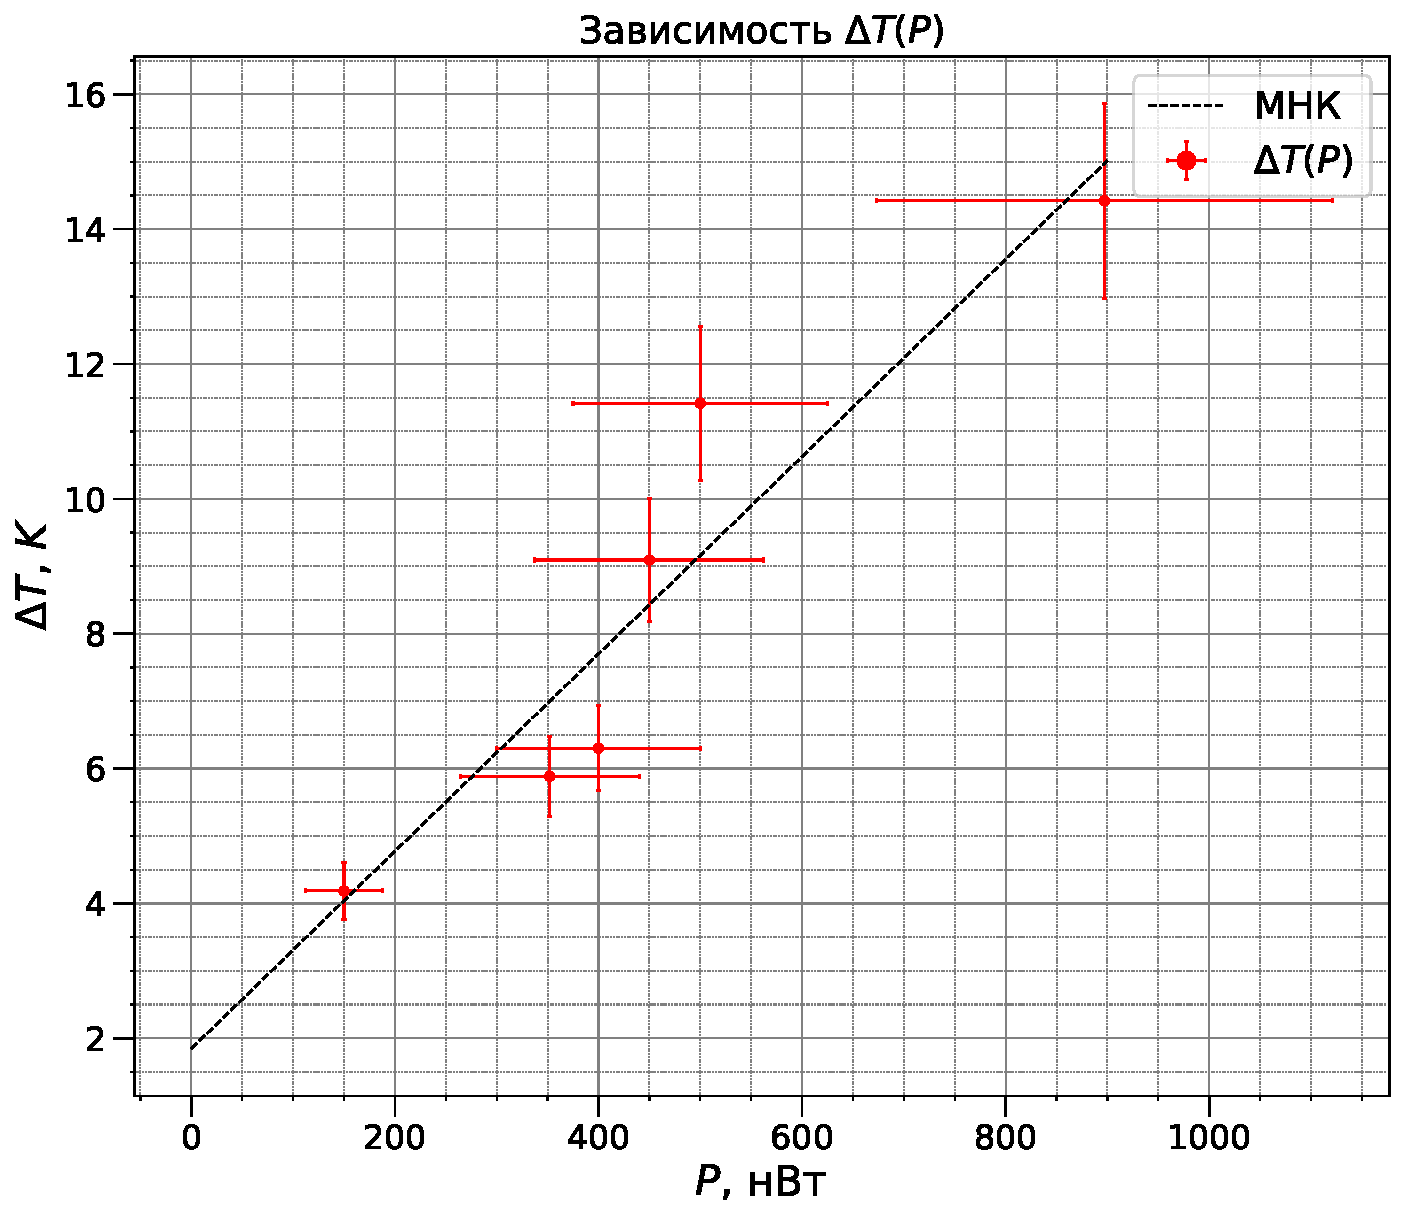
\includegraphics[width=1\textwidth]{5.11.8/T(P).pdf}
    \caption{График $\Delta T(P)$}
    \label{graph1}
\end{figure}

Далее, по формуле $\displaystyle L = \frac{R}{A}\times\frac{1}{T}$, считая температуру равно $300 \ K$ найдем постоянную Лоренца, которая составила $L = 3,60 \pm 0,68 \cdot 10^{-8}$ Вт$\cdot$Ом$\cdot$К$^{-2}$. Это сходится по порядку с табличными данными, которые говорят, что $L = 2,44 \cdot 10^{-8}$ Вт$\cdot$Ом$\cdot$К$^{-2}$.

\section{Выводы}

Была экспериментально определена величины постоянной Лоренца $\displaystyle L=\frac{\kappa}{T\sigma}$ (здесь $\kappa$ – коэффициент теплопроводности, $\sigma$ – проводимость, а $T$ —
абсолютная температура) при комнатной температуре для Латуни. Она составила $L = 3,60 \pm 0,68 \cdot 10^{-8}$ Вт$\cdot$Ом$\cdot$К$^{-2}$, что неплохо сходится с табличными данными (т.е. по порядку).

В процессе работы возникли очень большие погрешности определния разности температур из-за большого времени установления равновесия и неточности определения мощности из-за большой погрешности округления показателей напряжения на образце. Этим объясняется небольшое расхождение численного значения постоянной Лоренца с истинной.

\end{document}
